\apendice
\renewcommand\thechapter{\arabic{chapter}}

\chapter{Tabela Completa de \textit{Clusters} Espaciais}
\label{app:clusters}

A tabela apresenta todos os \textit{clusters} significativos da varredura em rodada única com teto duplo. $RR$ é o risco relativo da zona; os casos esperados são calculados sob o modelo de Poisson e a população média municipal do período.

\begingroup\fontsize{9}{11}\selectfont

\begin{xltabular}{\linewidth}{>{\centering\arraybackslash}X>{\centering\arraybackslash}X>{\centering\arraybackslash}X>{\centering\arraybackslash}X>{\centering\arraybackslash}X>{\centering\arraybackslash}X}
\caption{\label{tab:clusters_satscan_puro}\textit{Clusters} espaciais significativos de dengue detectados pela varredura espacial sem ajuste por covariáveis, Brasil, 2010--2025.}\\
\toprule
\textit{Cluster} & Qtd. municípios & Raio (km) & Casos obs. ($C_Z$) & Casos esp. ($E_Z$) & Risco relativo ($RR_Z$)\\
\midrule
\endfirsthead
\caption[]{\textit{Clusters} espaciais significativos de dengue detectados pela varredura espacial sem ajuste por covariáveis, Brasil, 2010--2025. \textit{(continuação)}}\\
\toprule
\textit{Cluster} & Qtd. municípios & Raio (km) & Casos obs. ($C_Z$) & Casos esp. ($E_Z$) & Risco relativo ($RR_Z$)\\
\midrule
\endhead
\midrule
\multicolumn{6}{r@{}}{\textit{(continuação)}}\\
\endfoot
\bottomrule
\endlastfoot
1 & 319 & 197,4 & 2.342.103 & 842.629 & 2,99\\
2 & 229 & 199,8 & 2.588.779 & 1.019.064 & 2,74\\
3 & 122 & 198,1 & 2.259.957 & 948.039 & 2,54\\
4 & 245 & 198,9 & 1.251.256 & 515.650 & 2,51\\
5 & 48 & 66,5 & 977.272 & 462.096 & 2,17\\
\addlinespace
6 & 136 & 129,0 & 382.821 & 176.908 & 2,18\\
7 & 38 & 99,0 & 528.559 & 288.913 & 1,85\\
8 & 8 & 43,5 & 221.354 & 85.286 & 2,61\\
9 & 43 & 165,6 & 196.827 & 76.218 & 2,60\\
10 & 23 & 197,6 & 251.787 & 128.381 & 1,97\\
\addlinespace
11 & 1 & 0,0 & 46.111 & 9.322 & 4,95\\
12 & 134 & 107,1 & 414.194 & 268.589 & 1,55\\
13 & 178 & 198,4 & 438.280 & 300.249 & 1,47\\
14 & 10 & 30,0 & 199.249 & 120.188 & 1,66\\
15 & 21 & 199,5 & 85.974 & 44.806 & 1,92\\
\addlinespace
16 & 36 & 186,0 & 117.247 & 68.871 & 1,71\\
17 & 10 & 30,5 & 155.307 & 99.551 & 1,56\\
18 & 61 & 191,0 & 120.223 & 75.308 & 1,60\\
19 & 3 & 58,5 & 78.666 & 44.450 & 1,77\\
20 & 3 & 14,1 & 64.151 & 34.479 & 1,86\\
\addlinespace
21 & 4 & 17,9 & 76.625 & 44.302 & 1,73\\
22 & 1 & 0,0 & 66.301 & 37.511 & 1,77\\
23 & 3 & 74,5 & 22.399 & 7.900 & 2,84\\
24 & 1 & 0,0 & 48.486 & 24.863 & 1,95\\
25 & 22 & 44,6 & 44.577 & 24.704 & 1,81\\
\addlinespace
26 & 3 & 36,6 & 36.003 & 19.051 & 1,89\\
27 & 1 & 0,0 & 124.442 & 90.308 & 1,38\\
28 & 1 & 0,0 & 37.737 & 21.788 & 1,73\\
29 & 1 & 0,0 & 49.428 & 30.782 & 1,61\\
30 & 17 & 147,4 & 87.943 & 64.309 & 1,37\\
\addlinespace
31 & 3 & 10,7 & 10.112 & 4.128 & 2,45\\
32 & 3 & 38,8 & 60.398 & 43.145 & 1,40\\
33 & 11 & 34,0 & 23.602 & 14.423 & 1,64\\
34 & 1 & 0,0 & 10.437 & 5.546 & 1,88\\
35 & 1 & 0,0 & 7.958 & 3.860 & 2,06\\
\addlinespace
36 & 1 & 0,0 & 9.754 & 5.296 & 1,84\\
37 & 9 & 32,7 & 13.904 & 8.844 & 1,57\\
38 & 1 & 0,0 & 15.621 & 10.214 & 1,53\\
39 & 13 & 144,7 & 31.514 & 23.650 & 1,33\\
40 & 6 & 142,6 & 15.500 & 10.294 & 1,51\\
\addlinespace
41 & 1 & 0,0 & 32.709 & 24.980 & 1,31\\
42 & 1 & 0,0 & 12.519 & 8.003 & 1,56\\
43 & 1 & 0,0 & 21.847 & 15.867 & 1,38\\
44 & 9 & 50,9 & 26.731 & 20.207 & 1,32\\
45 & 1 & 0,0 & 64.072 & 53.782 & 1,19\\
\addlinespace
46 & 1 & 0,0 & 6.714 & 3.835 & 1,75\\
47 & 3 & 15,3 & 4.319 & 2.117 & 2,04\\
48 & 2 & 18,8 & 6.542 & 3.760 & 1,74\\
49 & 1 & 0,0 & 2.875 & 1.199 & 2,40\\
50 & 1 & 0,0 & 10.723 & 7.039 & 1,52\\
\addlinespace
51 & 3 & 165,0 & 7.386 & 4.433 & 1,67\\
52 & 1 & 0,0 & 7.833 & 4.859 & 1,61\\
53 & 1 & 0,0 & 6.292 & 3.721 & 1,69\\
54 & 1 & 0,0 & 12.350 & 8.791 & 1,41\\
55 & 1 & 0,0 & 14.655 & 10.860 & 1,35\\
\addlinespace
56 & 1 & 0,0 & 5.561 & 3.392 & 1,64\\
57 & 2 & 26,7 & 4.984 & 2.982 & 1,67\\
58 & 3 & 16,9 & 5.483 & 3.419 & 1,60\\
59 & 1 & 0,0 & 2.350 & 1.128 & 2,08\\
60 & 5 & 35,0 & 12.871 & 9.609 & 1,34\\
\addlinespace
61 & 1 & 0,0 & 5.399 & 3.445 & 1,57\\
62 & 3 & 131,6 & 8.807 & 6.240 & 1,41\\
63 & 1 & 0,0 & 5.078 & 3.244 & 1,57\\
64 & 1 & 0,0 & 6.091 & 4.068 & 1,50\\
65 & 4 & 185,8 & 21.462 & 17.525 & 1,22\\
\addlinespace
66 & 1 & 0,0 & 10.515 & 7.872 & 1,34\\
67 & 3 & 108,2 & 11.469 & 8.742 & 1,31\\
68 & 1 & 0,0 & 12.048 & 9.292 & 1,30\\
69 & 1 & 0,0 & 2.211 & 1.172 & 1,89\\
70 & 1 & 0,0 & 8.522 & 6.323 & 1,35\\
\addlinespace
71 & 1 & 0,0 & 8.763 & 6.538 & 1,34\\
72 & 1 & 0,0 & 3.286 & 2.010 & 1,64\\
73 & 1 & 0,0 & 2.679 & 1.598 & 1,68\\
74 & 1 & 0,0 & 6.072 & 4.361 & 1,39\\
75 & 1 & 0,0 & 733 & 291 & 2,52\\
\addlinespace
76 & 1 & 0,0 & 2.514 & 1.603 & 1,57\\
77 & 1 & 0,0 & 4.585 & 3.309 & 1,39\\
78 & 3 & 99,8 & 5.520 & 4.171 & 1,32\\
79 & 1 & 0,0 & 2.848 & 1.954 & 1,46\\
80 & 1 & 0,0 & 10.807 & 8.972 & 1,20\\
\addlinespace
81 & 1 & 0,0 & 3.609 & 2.629 & 1,37\\
82 & 1 & 0,0 & 952 & 500 & 1,90\\
83 & 1 & 0,0 & 3.347 & 2.418 & 1,38\\
84 & 1 & 0,0 & 2.690 & 1.901 & 1,41\\
85 & 1 & 0,0 & 1.932 & 1.300 & 1,49\\
\addlinespace
86 & 1 & 0,0 & 7.733 & 6.387 & 1,21\\
87 & 5 & 63,8 & 11.486 & 9.883 & 1,16\\
88 & 2 & 11,9 & 63.457 & 59.585 & 1,07\\
89 & 1 & 0,0 & 2.955 & 2.210 & 1,34\\
90 & 1 & 0,0 & 3.571 & 2.767 & 1,29\\
\addlinespace
91 & 1 & 0,0 & 2.730 & 2.038 & 1,34\\
92 & 1 & 0,0 & 28.593 & 26.204 & 1,09\\
93 & 1 & 0,0 & 2.820 & 2.125 & 1,33\\
94 & 1 & 0,0 & 9.917 & 8.577 & 1,16\\
95 & 1 & 0,0 & 2.233 & 1.641 & 1,36\\
\addlinespace
96 & 5 & 24,8 & 10.747 & 9.437 & 1,14\\
97 & 1 & 0,0 & 847 & 528 & 1,60\\
98 & 1 & 0,0 & 3.901 & 3.166 & 1,23\\
99 & 1 & 0,0 & 1.424 & 1.000 & 1,42\\
100 & 1 & 0,0 & 1.067 & 719 & 1,48\\
\addlinespace
101 & 2 & 22,6 & 7.997 & 6.964 & 1,15\\
102 & 1 & 0,0 & 2.346 & 1.818 & 1,29\\
103 & 1 & 0,0 & 2.558 & 2.021 & 1,27\\
104 & 1 & 0,0 & 912 & 610 & 1,50\\
105 & 1 & 0,0 & 1.018 & 703 & 1,45\\
\addlinespace
106 & 1 & 0,0 & 783 & 515 & 1,52\\
107 & 5 & 20,4 & 12.755 & 11.583 & 1,10\\
108 & 2 & 30,9 & 2.562 & 2.072 & 1,24\\
109 & 1 & 0,0 & 2.585 & 2.097 & 1,23\\
110 & 1 & 0,0 & 2.598 & 2.124 & 1,22\\
\addlinespace
111 & 1 & 0,0 & 449 & 274 & 1,64\\
112 & 1 & 0,0 & 1.417 & 1.087 & 1,30\\
113 & 1 & 0,0 & 1.122 & 857 & 1,31\\
114 & 1 & 0,0 & 710 & 511 & 1,39\\
115 & 1 & 0,0 & 928 & 700 & 1,33\\
\addlinespace
116 & 1 & 0,0 & 17.764 & 16.711 & 1,06\\
117 & 1 & 0,0 & 6.339 & 5.731 & 1,11\\
118 & 1 & 0,0 & 462 & 323 & 1,43\\
119 & 4 & 14,2 & 2.039 & 1.734 & 1,18\\
120 & 1 & 0,0 & 862 & 673 & 1,28\\
\addlinespace
121 & 1 & 0,0 & 407 & 284 & 1,43\\
122 & 1 & 0,0 & 2.218 & 1.935 & 1,15\\
123 & 1 & 0,0 & 800 & 639 & 1,25\\
124 & 1 & 0,0 & 802 & 645 & 1,24\\
125 & 1 & 0,0 & 1.420 & 1.210 & 1,17\\
\addlinespace
126 & 1 & 0,0 & 2.587 & 2.301 & 1,12\\
127 & 1 & 0,0 & 598 & 471 & 1,27\\
128 & 1 & 0,0 & 9.754 & 9.214 & 1,06\\
129 & 1 & 0,0 & 1.802 & 1.599 & 1,13\\*
\end{xltabular}
\endgroup{}


\par\vspace{0.4em}
\parbox{\linewidth}{\footnotesize\textit{Nota:} A tabela não apresenta município polo; a ordenação segue a coleção reportada pelo programa. Valores de casos e risco relativo são os estimados para 2010--2025.}

\chapter{Tabela Completa de \textit{Clusters} com Ajuste Térmico}
\label{app:clusters_termica}

A tabela apresenta as zonas da varredura em rodada única com padronização indireta pelos tercis de dias sob onda de calor. Os valores devem ser interpretados como resultado exploratório da análise ajustada, não como estimativas de efeito causal da temperatura.

\begingroup\fontsize{9}{11}\selectfont

\begin{xltabular}{\linewidth}{>{\centering\arraybackslash}X>{\centering\arraybackslash}X>{\centering\arraybackslash}X>{\centering\arraybackslash}X>{\centering\arraybackslash}X>{\centering\arraybackslash}X}
\caption{\label{tab:clusters_satscan_termica}\textit{Clusters} espaciais significativos de dengue detectados pela varredura espacial sob padronização indireta pelos tercis de dias em onda de calor, Brasil, 2010--2025.}\\
\toprule
\textit{Cluster} & Qtd. municípios & Raio (km) & Casos obs. ($C_Z$) & Casos esp. ($E_Z$) & Risco relativo ($RR_Z$)\\
\midrule
\endfirsthead
\caption[]{\textit{Clusters} espaciais significativos de dengue detectados pela varredura espacial sob padronização indireta pelos tercis de dias em onda de calor, Brasil, 2010--2025. \textit{(continuação)}}\\
\toprule
\textit{Cluster} & Qtd. municípios & Raio (km) & Casos obs. ($C_Z$) & Casos esp. ($E_Z$) & Risco relativo ($RR_Z$)\\
\midrule
\endhead
\midrule
\multicolumn{6}{r@{}}{\textit{(continuação)}}\\
\endfoot
\bottomrule
\endlastfoot
1 & 362 & 199,5 & 2.967.585 & 1.533.663 & 2,08\\
2 & 335 & 199,3 & 3.232.573 & 1.868.613 & 1,86\\
3 & 3 & 18,8 & 810.059 & 344.386 & 2,40\\
4 & 245 & 198,9 & 1.267.677 & 663.178 & 1,97\\
5 & 38 & 99,0 & 528.559 & 185.110 & 2,90\\
\addlinespace
6 & 26 & 70,8 & 408.413 & 146.361 & 2,82\\
7 & 45 & 82,8 & 368.333 & 160.010 & 2,32\\
8 & 105 & 197,5 & 461.706 & 270.945 & 1,72\\
9 & 1 & 0,0 & 46.111 & 10.214 & 4,52\\
10 & 2 & 121,0 & 130.373 & 58.493 & 2,24\\
\addlinespace
11 & 9 & 41,3 & 87.296 & 33.935 & 2,58\\
12 & 2 & 14,3 & 128.239 & 60.392 & 2,13\\
13 & 75 & 198,8 & 531.276 & 380.155 & 1,41\\
14 & 1 & 0,0 & 48.486 & 15.930 & 3,05\\
15 & 15 & 83,1 & 67.798 & 28.962 & 2,35\\
\addlinespace
16 & 58 & 166,2 & 1.011.751 & 853.839 & 1,19\\
17 & 3 & 38,8 & 60.398 & 28.517 & 2,12\\
18 & 24 & 73,4 & 69.719 & 36.928 & 1,89\\
19 & 20 & 49,1 & 38.268 & 18.156 & 2,11\\
20 & 23 & 81,8 & 175.388 & 131.149 & 1,34\\
\addlinespace
21 & 33 & 57,7 & 57.425 & 34.354 & 1,67\\
22 & 3 & 10,7 & 10.112 & 2.645 & 3,82\\
23 & 1 & 0,0 & 225.675 & 178.132 & 1,27\\
24 & 6 & 19,3 & 109.745 & 79.792 & 1,38\\
25 & 11 & 125,9 & 214.584 & 172.820 & 1,24\\
\addlinespace
26 & 10 & 105,0 & 40.851 & 24.267 & 1,68\\
27 & 8 & 15,9 & 55.731 & 36.793 & 1,52\\
28 & 24 & 101,0 & 65.264 & 44.734 & 1,46\\
29 & 1 & 0,0 & 76.901 & 55.764 & 1,38\\
30 & 1 & 0,0 & 12.350 & 5.632 & 2,19\\
\addlinespace
31 & 3 & 74,5 & 22.399 & 12.764 & 1,76\\
32 & 3 & 18,8 & 7.000 & 2.643 & 2,65\\
33 & 5 & 15,1 & 17.944 & 10.716 & 1,67\\
34 & 13 & 93,9 & 26.549 & 17.986 & 1,48\\
35 & 14 & 83,7 & 41.877 & 30.847 & 1,36\\
\addlinespace
36 & 2 & 26,7 & 4.984 & 1.911 & 2,61\\
37 & 1 & 0,0 & 6.091 & 2.607 & 2,34\\
38 & 1 & 0,0 & 5.399 & 2.207 & 2,45\\
39 & 13 & 180,0 & 58.224 & 45.575 & 1,28\\
40 & 2 & 37,1 & 13.503 & 8.303 & 1,63\\
\addlinespace
41 & 8 & 100,7 & 35.309 & 26.444 & 1,34\\
42 & 1 & 0,0 & 9.754 & 5.803 & 1,68\\
43 & 3 & 21,8 & 11.986 & 7.657 & 1,57\\
44 & 1 & 0,0 & 3.722 & 1.639 & 2,27\\
45 & 1 & 0,0 & 3.024 & 1.259 & 2,40\\
\addlinespace
46 & 2 & 56,0 & 6.258 & 3.554 & 1,76\\
47 & 1 & 0,0 & 2.514 & 1.027 & 2,45\\
48 & 2 & 12,2 & 8.054 & 5.114 & 1,58\\
49 & 14 & 26,2 & 19.990 & 15.135 & 1,32\\
50 & 1 & 0,0 & 2.955 & 1.416 & 2,09\\
\addlinespace
51 & 1 & 0,0 & 2.730 & 1.306 & 2,09\\
52 & 4 & 35,2 & 14.209 & 10.570 & 1,34\\
53 & 4 & 20,5 & 3.322 & 1.745 & 1,90\\
54 & 1 & 0,0 & 10.723 & 7.713 & 1,39\\
55 & 2 & 20,6 & 7.618 & 5.158 & 1,48\\
\addlinespace
56 & 1 & 0,0 & 2.233 & 1.052 & 2,12\\
57 & 2 & 15,5 & 22.419 & 18.095 & 1,24\\
58 & 1 & 0,0 & 2.558 & 1.295 & 1,98\\
59 & 1 & 0,0 & 2.585 & 1.344 & 1,92\\
60 & 3 & 74,7 & 16.175 & 12.662 & 1,28\\
\addlinespace
61 & 1 & 0,0 & 2.378 & 1.206 & 1,97\\
62 & 1 & 0,0 & 2.774 & 1.571 & 1,77\\
63 & 1 & 0,0 & 72.558 & 65.610 & 1,11\\
64 & 1 & 0,0 & 1.424 & 641 & 2,22\\
65 & 1 & 0,0 & 2.827 & 1.668 & 1,70\\
\addlinespace
66 & 1 & 0,0 & 4.700 & 3.161 & 1,49\\
67 & 1 & 0,0 & 2.180 & 1.220 & 1,79\\
68 & 2 & 27,0 & 2.552 & 1.561 & 1,63\\
69 & 2 & 14,9 & 16.311 & 13.588 & 1,20\\
70 & 1 & 0,0 & 3.286 & 2.202 & 1,49\\
\addlinespace
71 & 1 & 0,0 & 10.515 & 8.625 & 1,22\\
72 & 1 & 0,0 & 8.522 & 6.928 & 1,23\\
73 & 1 & 0,0 & 8.763 & 7.163 & 1,22\\
74 & 1 & 0,0 & 800 & 409 & 1,95\\
75 & 1 & 0,0 & 4.360 & 3.331 & 1,31\\
\addlinespace
76 & 1 & 0,0 & 1.274 & 767 & 1,66\\
77 & 1 & 0,0 & 952 & 548 & 1,74\\
78 & 1 & 0,0 & 951 & 549 & 1,73\\
79 & 1 & 0,0 & 10.351 & 8.868 & 1,17\\
80 & 1 & 0,0 & 5.459 & 4.407 & 1,24\\
\addlinespace
81 & 1 & 0,0 & 10.437 & 8.961 & 1,16\\
82 & 1 & 0,0 & 2.070 & 1.496 & 1,38\\
83 & 1 & 0,0 & 1.476 & 1.006 & 1,47\\
84 & 1 & 0,0 & 6.332 & 5.301 & 1,19\\
85 & 1 & 0,0 & 1.837 & 1.312 & 1,40\\
\addlinespace
86 & 1 & 0,0 & 1.141 & 752 & 1,52\\
87 & 1 & 0,0 & 3.609 & 2.881 & 1,25\\
88 & 1 & 0,0 & 3.347 & 2.650 & 1,26\\
89 & 1 & 0,0 & 1.849 & 1.377 & 1,34\\
90 & 1 & 0,0 & 525 & 296 & 1,77\\
\addlinespace
91 & 1 & 0,0 & 3.270 & 2.632 & 1,24\\
92 & 3 & 38,0 & 10.512 & 9.346 & 1,12\\
93 & 1 & 0,0 & 565 & 334 & 1,69\\
94 & 1 & 0,0 & 2.819 & 2.262 & 1,25\\
95 & 1 & 0,0 & 687 & 439 & 1,57\\
\addlinespace
96 & 3 & 18,5 & 6.536 & 5.746 & 1,14\\
97 & 1 & 0,0 & 2.106 & 1.678 & 1,26\\
98 & 2 & 19,9 & 3.308 & 2.771 & 1,19\\
99 & 1 & 0,0 & 658 & 437 & 1,51\\
100 & 1 & 0,0 & 10.807 & 9.830 & 1,10\\
\addlinespace
101 & 1 & 0,0 & 1.067 & 787 & 1,36\\
102 & 1 & 0,0 & 1.295 & 985 & 1,32\\
103 & 1 & 0,0 & 681 & 466 & 1,46\\
104 & 1 & 0,0 & 1.148 & 862 & 1,33\\
105 & 2 & 27,7 & 2.410 & 1.989 & 1,21\\
\addlinespace
106 & 1 & 0,0 & 3.201 & 2.721 & 1,18\\
107 & 1 & 0,0 & 373 & 229 & 1,63\\
108 & 1 & 0,0 & 439 & 281 & 1,56\\
109 & 1 & 0,0 & 1.884 & 1.532 & 1,23\\
110 & 1 & 0,0 & 1.049 & 795 & 1,32\\
\addlinespace
111 & 1 & 0,0 & 1.018 & 770 & 1,32\\
112 & 1 & 0,0 & 502 & 339 & 1,48\\
113 & 1 & 0,0 & 625 & 443 & 1,41\\
114 & 1 & 0,0 & 2.625 & 2.242 & 1,17\\
115 & 1 & 0,0 & 869 & 664 & 1,31\\
\addlinespace
116 & 1 & 0,0 & 1.167 & 928 & 1,26\\
117 & 1 & 0,0 & 2.211 & 1.893 & 1,17\\
118 & 1 & 0,0 & 1.608 & 1.349 & 1,19\\
119 & 1 & 0,0 & 2.226 & 1.924 & 1,16\\
120 & 2 & 34,8 & 7.542 & 6.977 & 1,08\\
\addlinespace
121 & 1 & 0,0 & 6.714 & 6.196 & 1,08\\
122 & 1 & 0,0 & 1.417 & 1.191 & 1,19\\
123 & 2 & 45,5 & 2.380 & 2.095 & 1,14\\
124 & 1 & 0,0 & 288 & 200 & 1,44\\
125 & 1 & 0,0 & 1.122 & 938 & 1,20\\
\addlinespace
126 & 1 & 0,0 & 928 & 767 & 1,21\\
127 & 1 & 0,0 & 3.627 & 3.337 & 1,09\\
128 & 1 & 0,0 & 1.141 & 984 & 1,16\\*
\end{xltabular}
\endgroup{}


\par\vspace{0.4em}
\parbox{\linewidth}{\footnotesize\textit{Nota:} A tabela não apresenta município polo; a ordenação segue a coleção reportada pelo programa. Valores de casos, expectativa e risco relativo são os estimados para 2010--2025.}

\chapter{Pranchas de zonas e de risco relativo}
\label{app:pranchas}

As pranchas reúnem, em uma página cada, os oito mapas de zonas significativas de 2010--2025 (Figura~\ref{fig:prancha_clusters}), os oito do cenário sem 2024 (Figura~\ref{fig:prancha_clusters_sem2024}) e os seis mapas de risco relativo das demais formulações (Figura~\ref{fig:prancha_rr}). O desenho é compacto: uma escala gráfica e uma rosa dos ventos por prancha, painéis em ordem de leitura e sem contorno municipal individual. A leitura município a município deve usar as figuras do corpo e as tabelas de \textit{clusters} dos Apêndices~\ref{app:clusters} e \ref{app:clusters_termica}.

\begin{figure}[H]
    \centering
    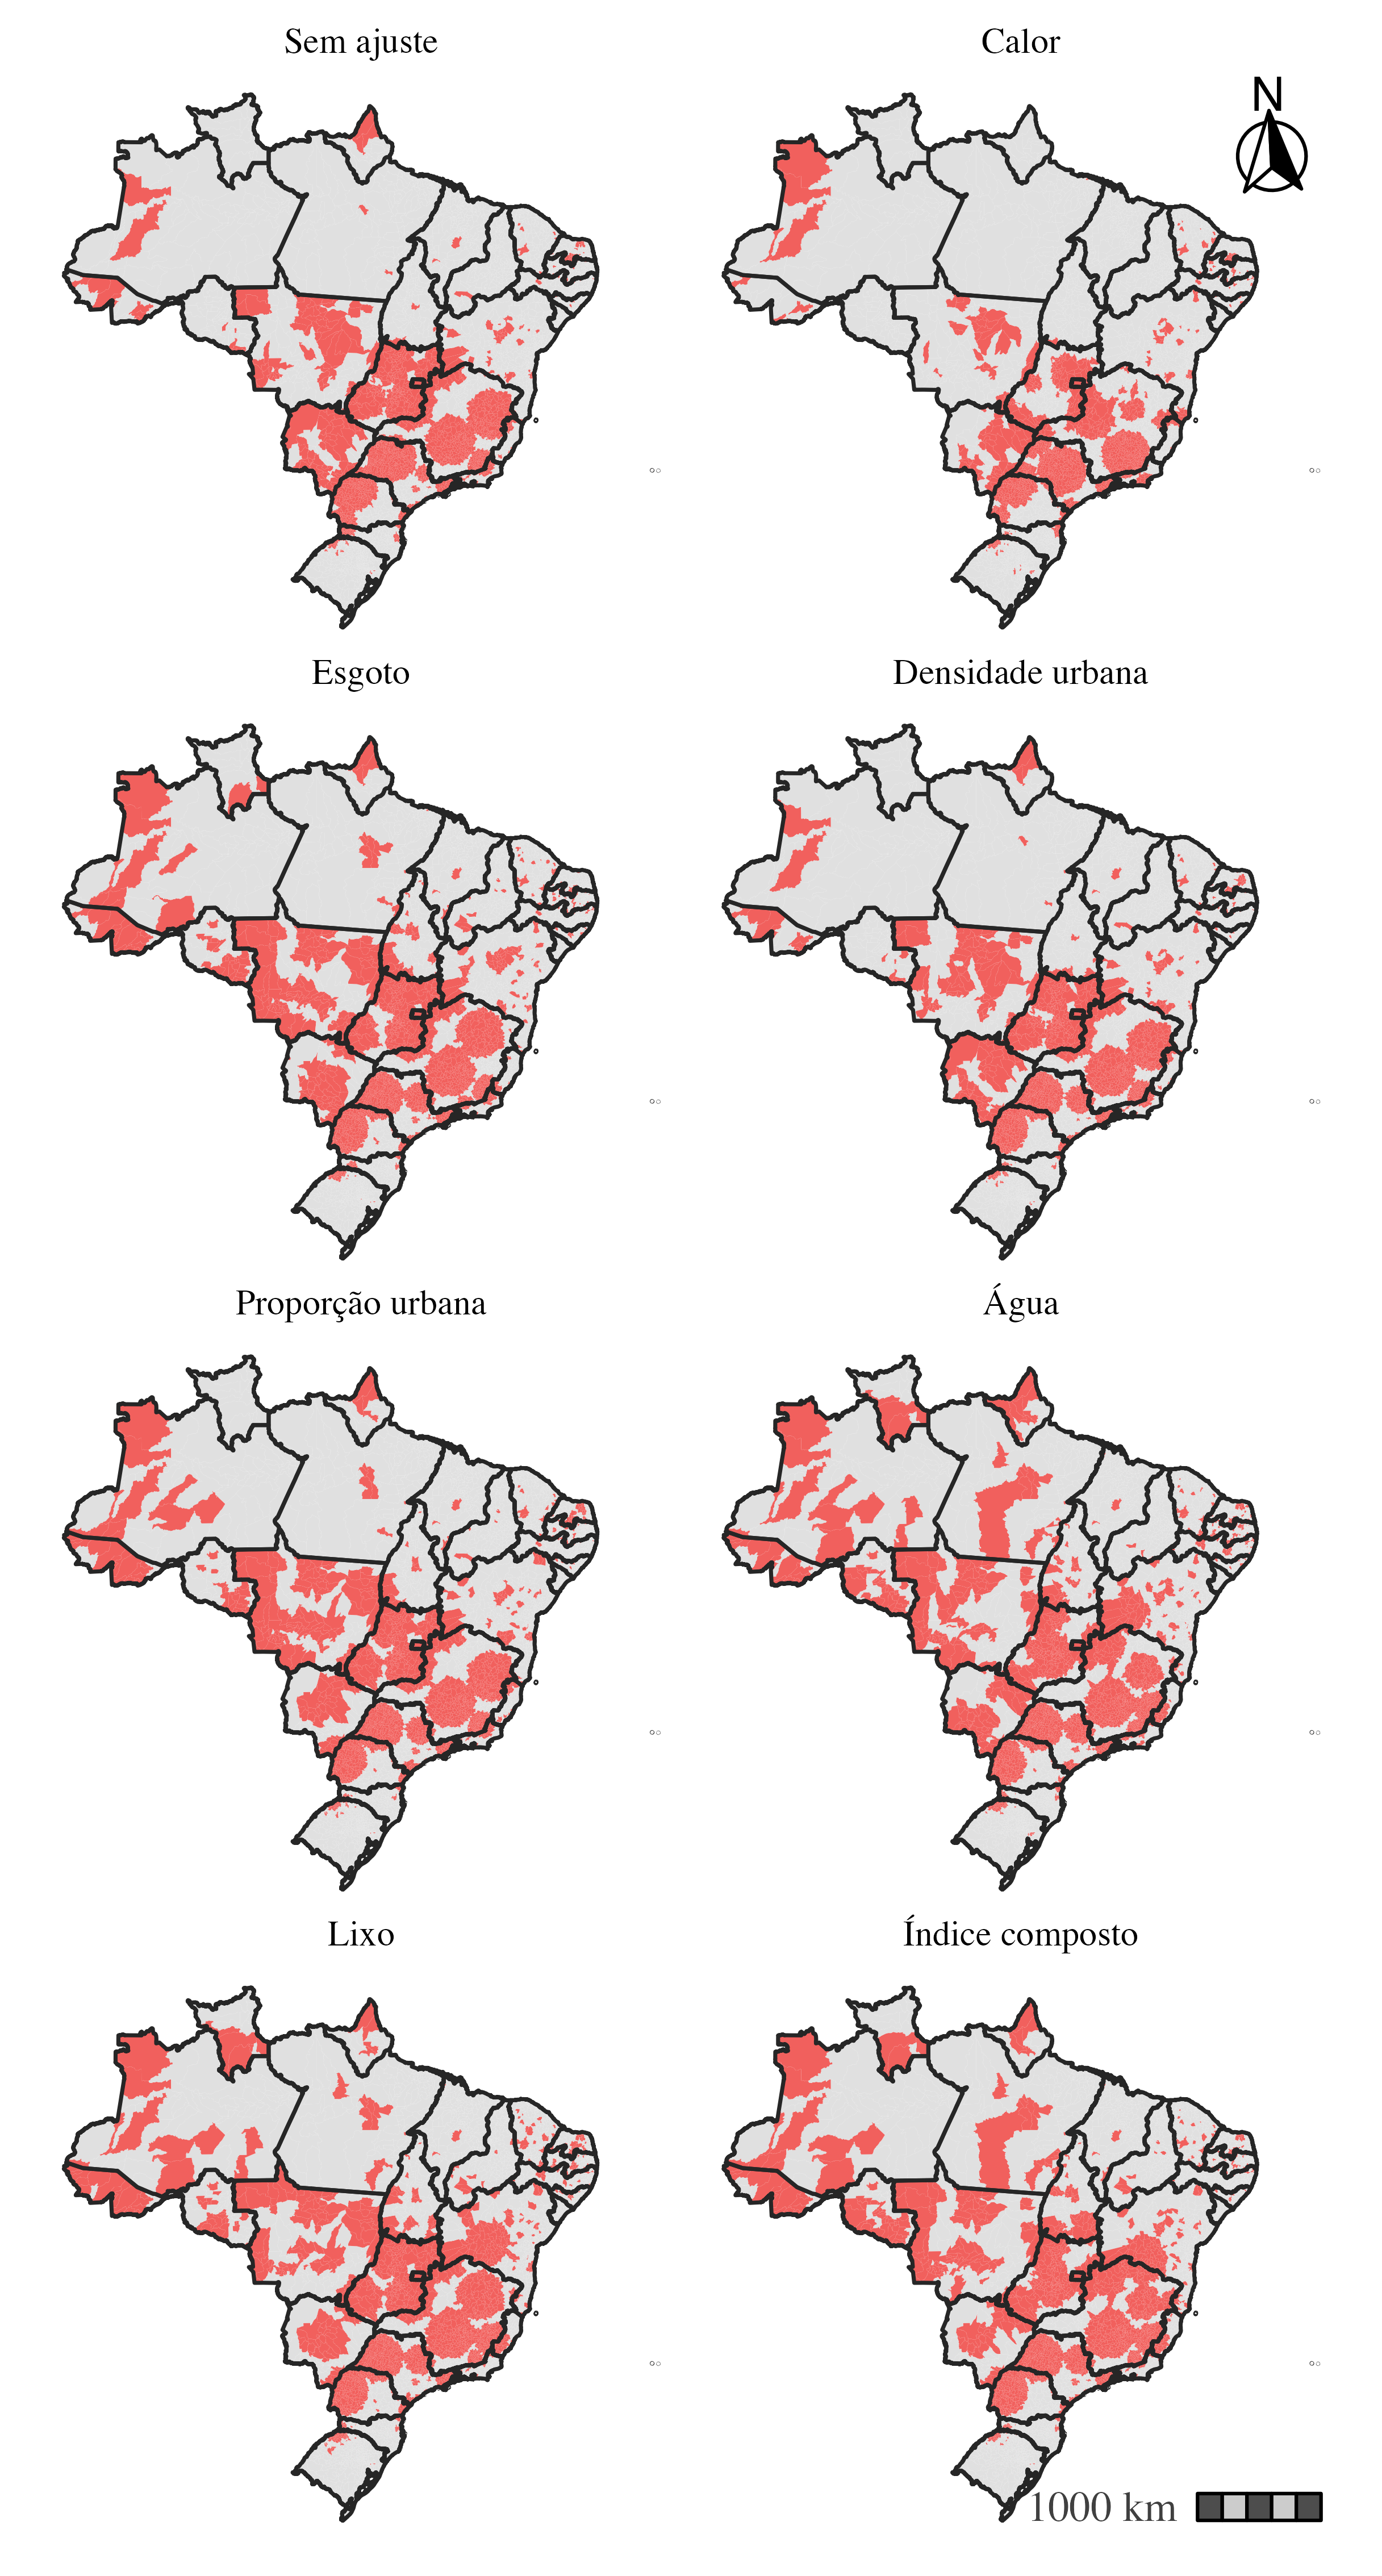
\includegraphics[width=0.60\textwidth]{fig_prancha_clusters_completo.png}
    \caption{Zonas significativas de alto risco por formulação da varredura espacial, Brasil, 2010--2025, em ordem de leitura: sem ajuste, calor, esgoto, densidade urbana, proporção urbana, água, lixo e índice composto. Fontes: SINAN e IBGE.}
    \label{fig:prancha_clusters}
    \vspace{0.3em}
    {\footnotesize\noindent\textit{Nota:} Em laranja, municípios em zonas com nível de 5\%; em cinza, municípios fora de zonas. Todas as formulações usam o mesmo limite de 16\% da população e 200~km, com 999 réplicas e reporte sem sobreposição geográfica.\par}
\end{figure}

\begin{figure}[H]
    \centering
    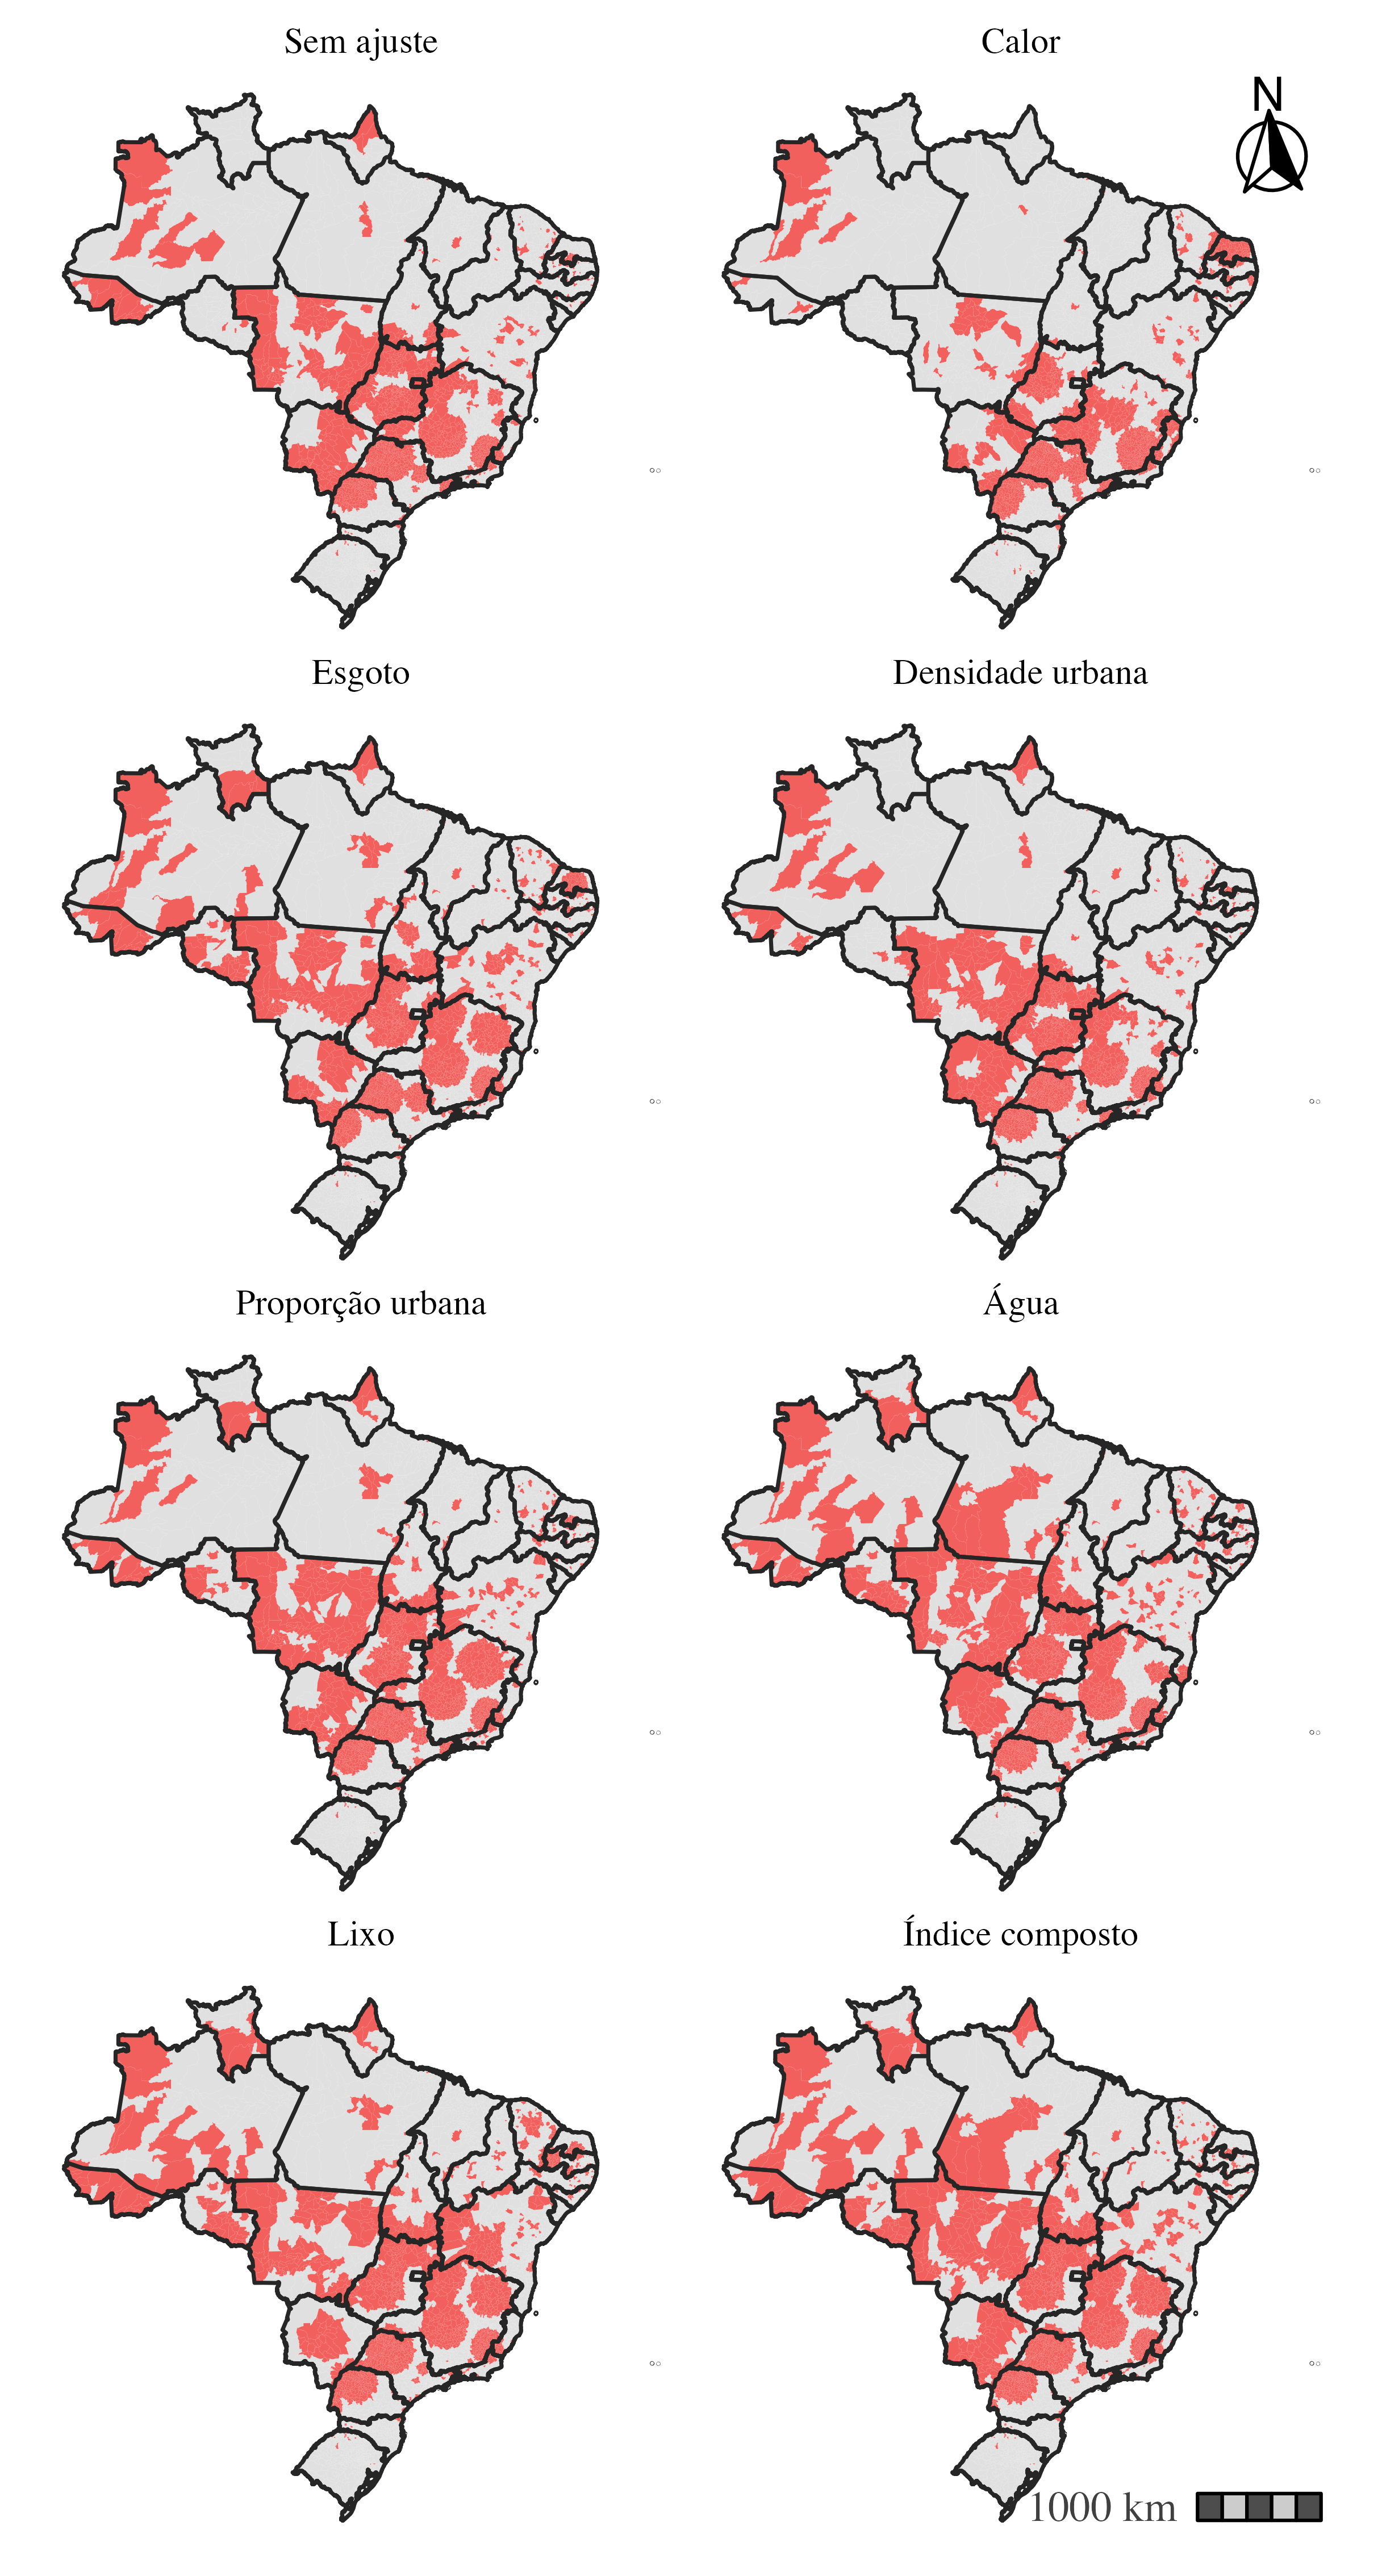
\includegraphics[width=0.60\textwidth]{fig_prancha_clusters_sem2024.png}
    \caption{Zonas significativas de alto risco por formulação da varredura espacial sem os casos de 2024, Brasil, 2010--2023 e 2025, em ordem de leitura: sem ajuste, calor, esgoto, densidade urbana, proporção urbana, água, lixo e índice composto. Fontes: SINAN e IBGE.}
    \label{fig:prancha_clusters_sem2024}
    \vspace{0.3em}
    {\footnotesize\noindent\textit{Nota:} Mesma codificação de cor e mesma configuração da prancha anterior; o painel sem 2024 reúne 15.664.546 casos.\par}
\end{figure}

\begin{figure}[H]
    \centering
    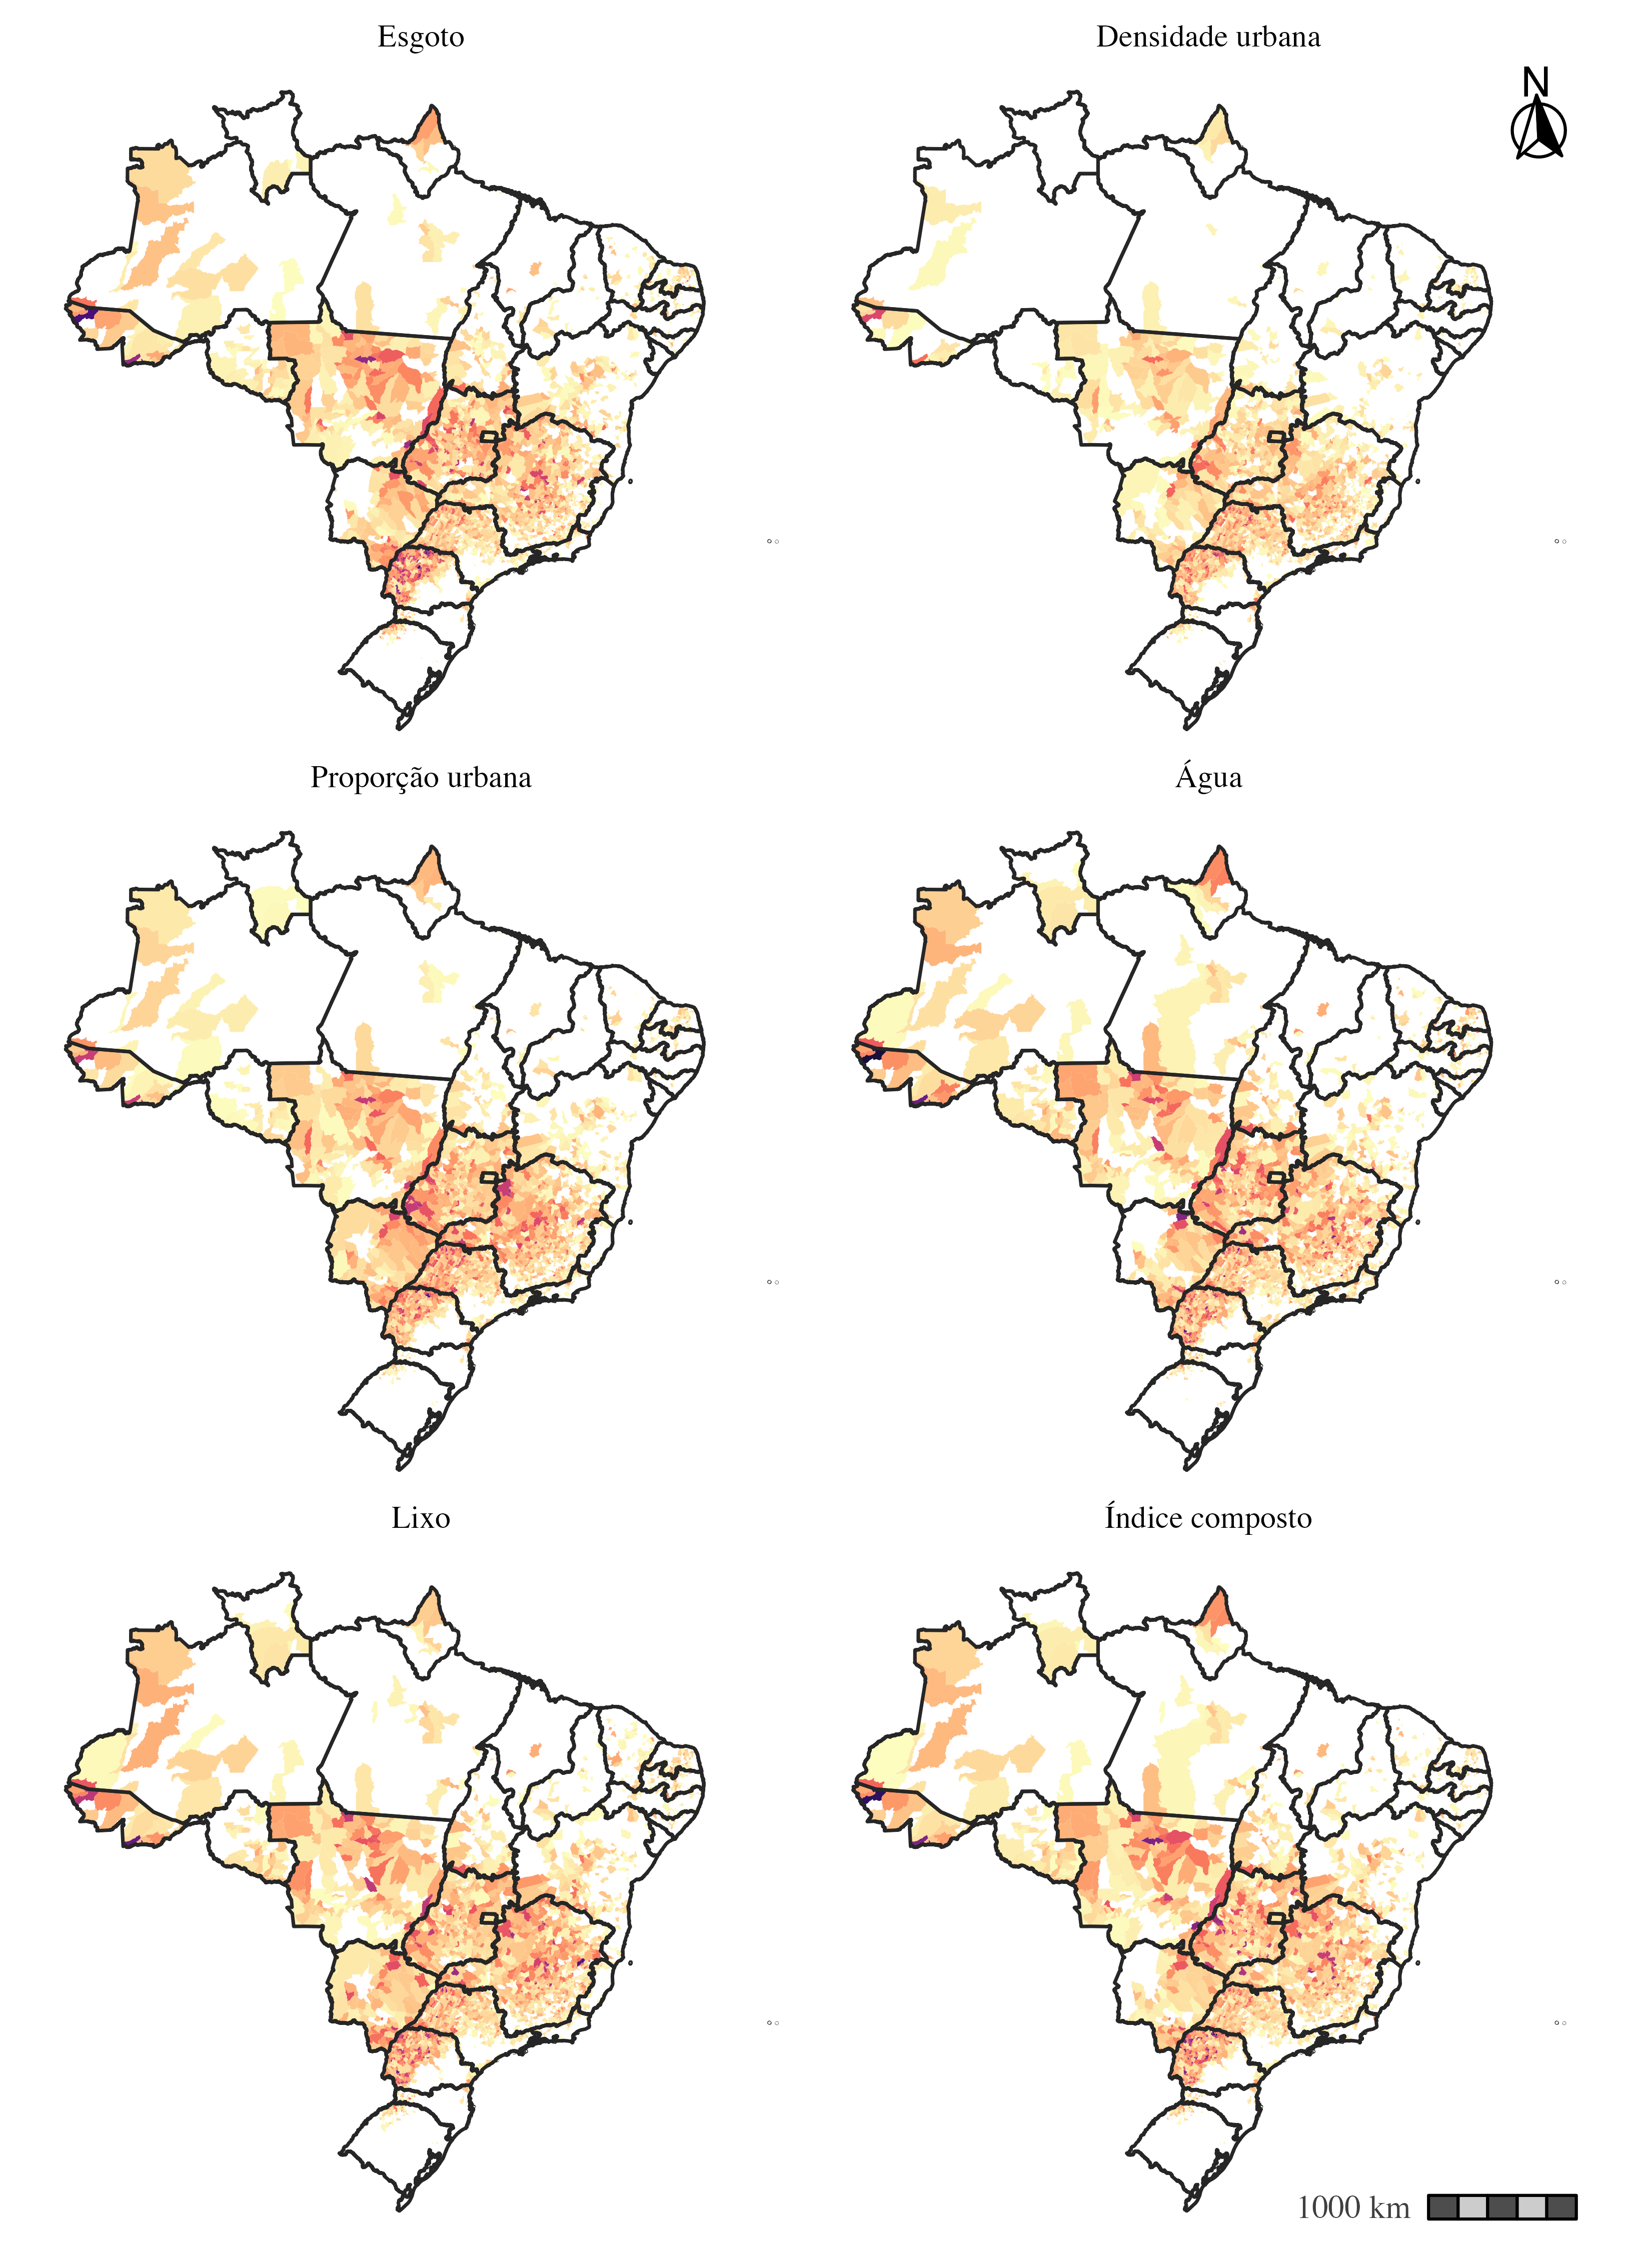
\includegraphics[width=0.86\textwidth]{fig_prancha_rr_completo.png}
    \caption{Risco relativo municipal estimado pela varredura espacial sob os ajustes por esgoto, densidade urbana, proporção urbana, água, lixo e índice composto (ordem de leitura), Brasil, 2010--2025. Fontes: SINAN e IBGE.}
    \label{fig:prancha_rr}
    \vspace{0.3em}
    {\footnotesize\noindent\textit{Nota:} Tons mais escuros indicam risco relativo mais alto, na escala comum às seis formulações, de 1,0 a 11,9; em branco, municípios com $RR \le 1{,}0$. Os dois primeiros modelos constam da Figura~\ref{fig:mapas_rr}.\par}
